\documentclass{article}

\usepackage{hw}
\usepackage{bm}
\usepackage{amsmath}
\usepackage{graphicx}
\usepackage[colorlinks=true,urlcolor=blue]{hyperref}
\usepackage{geometry}
\geometry{margin=1in}
\usepackage{multicol}
\usepackage{paralist}
\usepackage{todonotes}
\setlength{\marginparwidth}{2.15cm}
\usepackage{booktabs}
\usepackage{enumitem}
\usepackage{amsmath}
\usepackage{bm}
\usepackage{cleveref}
\usepackage{amsmath}

%\DeclareMathOperator*{\argmin}{arg\,min}
%\DeclareMathOperator*{\argmax}{arg\,max}

\def \issoln {1}

% Some commands to allow solutions to be embedded in the assignment file.
\ifcsname issoln\endcsname \else \def\issoln{0} \fi
\newcommand{\soln}[1]
{
  \if\issoln 1
  \textbf{Solution:}
  #1
  \fi
}

\begin{document}

\section*{}
\begin{center}
  \centerline{\textsc{\LARGE Homework Assignment 1{\if\issoln 1 Solutions \else \fi}}}
  \vspace{1em}
  \textsc{\large CMU 15-745: Optimizing Compilers (Spring 2015)} \\
  \vspace{3em}
  \centerline{\large{Joy Arulraj (jarulraj), Nisarg Shah (nkshah)}}
  \vspace{1em}
\end{center}

\section{Register Allocation}

The annotated CFG and the associated interference graph are shown below. 

We first identify the live ranges of all the variables. We split
pseudo-registers into live ranges to create an interference graph that
is easier to color.

We observe that the graph has a 5-clique comprising of $\{y, x_2, s_1, t, u \}$.
Hence, there is no possible 4-coloring for the graph.

We then compute the spilling cost for all the variables involved in the clique.
We note that either $x_2$ or $u$ can be spilled with minimal cost.
After spilling, say $u$, we provide a 4-coloring of the graph in the figure.
Thus, it is possible to allocate the variables in this case to 4 physical
registers after spilling $u$.

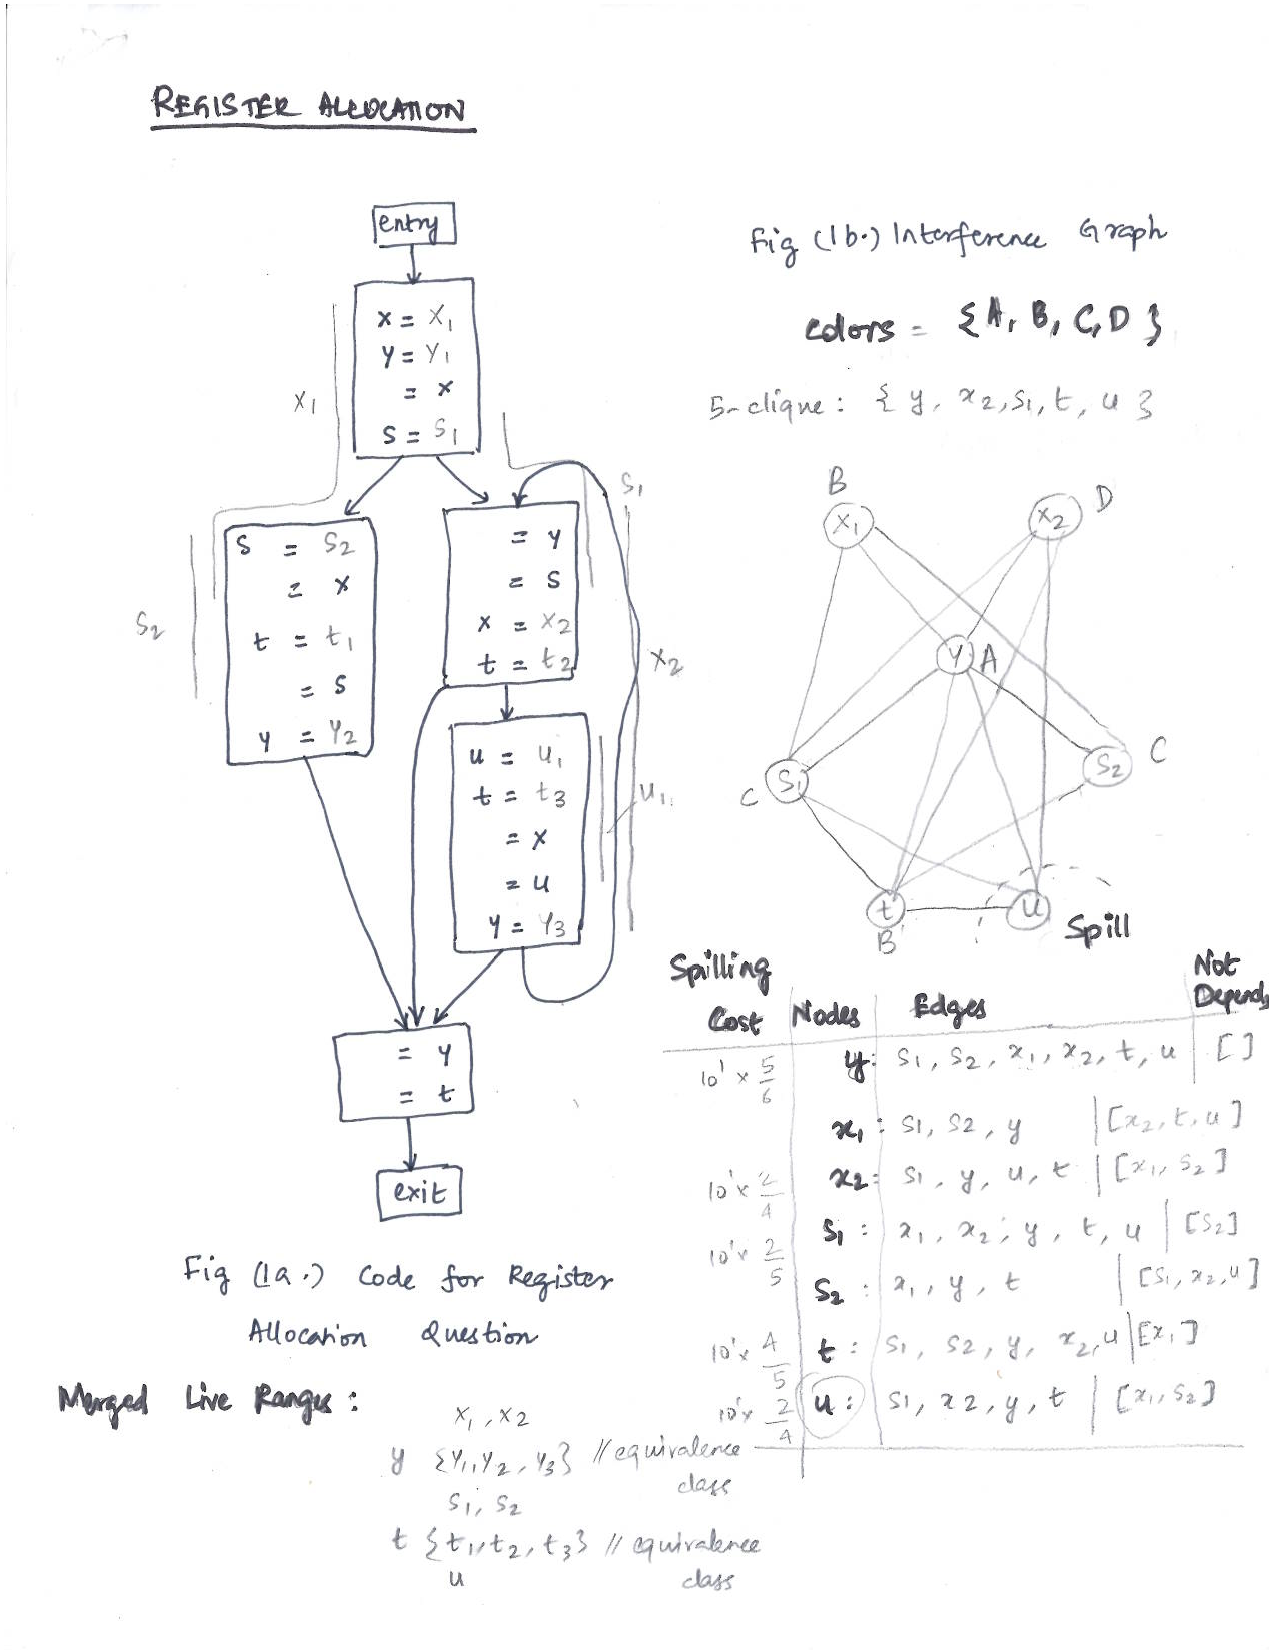
\includepdf[scale=0.7, pages={-}]{images/Q2.pdf}


\end{document}
